%\documentclass[12pt,serif]{beamer}
%\documentclass[tikz,12pt,svgnames]{beamer}
\documentclass[table,handout,tikz,12pt,svgnames]{beamer}
\usepackage{CM-preamble}
\subtitle{\Huge Listes}
%\date{5 février 2016}
\date{CM2}

\begin{document}

\begin{frame}
	\titlepage
\end{frame}

\begin{frame}[fragile=singleslide]
	\frametitle{Structures de Données}
		\begin{block}{Représentation de collections d'informations en fonction de :}
			\begin{itemize}
			\item traitements à privilégier
			\item contraintes
			\begin{itemize}
				\item espace disponible / temps d'éxecution
				\item outils disponibles (selon les différents langages)
			\end{itemize}
			\item propriétés
			\begin{itemize}
				\item relations d'ordre ?
				\item taux de dynamicité
				\item taille des informations
			\end{itemize}
		\end{itemize}
		\end{block}
\end{frame}

\begin{frame}[fragile=singleslide]
	\frametitle{Structures de Données}
	\begin{block}{Traitements typiques}
		\begin{itemize}
			\item Tris
			\item Recherche d'informations
			\begin{itemize}
				\item Par position: e.g., le kième élément
				\item Par valeur (associative) : $v \in C / P(v)$
			\end{itemize}
			\item Mises à jour
			\begin{itemize}
				\item Ajout
				\item Suppression
				\item Modification $\Rightarrow$ recherche
			\end{itemize}
		\end{itemize}
	\end{block}
\end{frame}

\begin{frame}[fragile=singleslide]
	\frametitle{Structures de Données:\\Classification des SD}
%	\begin{block}{}
		{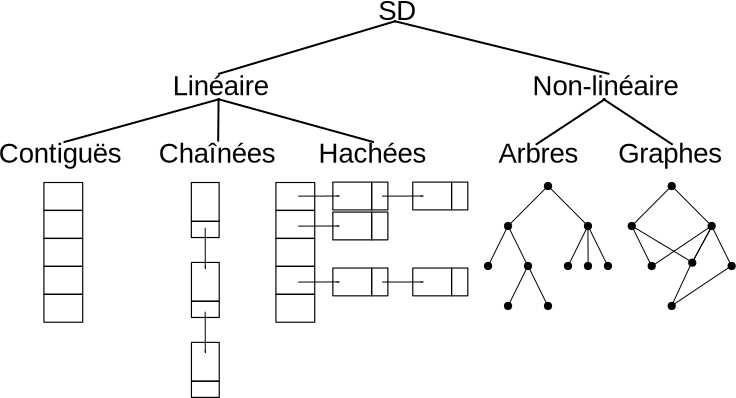
\includegraphics[scale=0.550]{../common-images/classification_sd.pdf}}
%	\end{block}
\end{frame}

\begin{frame}[fragile=singleslide]
	\frametitle{Structures de Données:\\Analyse des besoins}
	\begin{block}{}
		\begin{itemize}
			\item Identification des informations et de leurs caractéristiques
			\item Identification des opérations (recherche, ajout, suppression, ...)
			\item Opérations à privilégier ?
			\item Etude des représentations possibles (structures de données), avec méthodes de résolution et coûts associés
			\item Choix de la structure en fonction des coûts
		\end{itemize}
	\end{block}
\end{frame}


\begin{frame}[fragile=singleslide]
	\frametitle{Les listes contiguës}
	\begin{block}{Structures de données contiguës}
		\begin{itemize}
			\item Autorisent accès direct et calculé
			\begin{itemize}
				\item Déjà vu : tableaux
			\end{itemize}
		\end{itemize}
	\end{block}
	\begin{block}{Représentation}
	\vspace{0.7cm}
	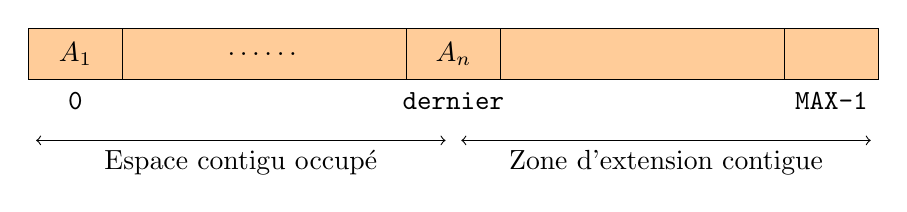
\begin{tikzpicture}
	% size of each node
	\def\sz{6.5mm}
	\def\szwidth{12mm}
	\def\offset{0.6}
	% node style definition
	\tikzstyle{block} = [draw, fill=orange!40, rectangle, minimum height=\sz, minimum width=\sz ];
	\tikzstyle{rect} = [draw, fill=orange!40, rectangle, minimum height=\sz, minimum width=\szwidth ];
	\tikzstyle{rect2} = [draw, fill=orange!40, rectangle, minimum height=\sz, minimum width=\szwidth*3 ];
	\tikzstyle{indices} = [rectangle, minimum height=\sz, minimum width=\szwidth ];
	\tikzstyle{plain} = [draw=none,fill=none];
	% array element definition
	\def\dateone{$A_0$,\ldots \ldots,$A_n$,,};
	\def\datetwo{0,,dernier,,MAX-1};
	%\def\x{0}; % x pos of arr
	%\def\y{0}; % y pos of arr
	\newcounter{ind};
	\setcounter{ind}{0};
%	\node[plain] { x };
	\node[rect] (first) at (0*\szwidth,\offset) { $A_1$ };
	\node[rect2] at (2*\szwidth,\offset) { \ldots\ldots };
	\node[rect] (middle) at (4*\szwidth,\offset) { $A_n$ };
	\node[rect2] at (6*\szwidth,\offset) {  };
	\node[rect] (last) at (8*\szwidth,\offset) {  };	
	\node[indices] at (0*\szwidth,0) { \texttt{0} };
	\node[indices] at (2*\szwidth,0) {  };
	\node[indices] at (4*\szwidth,0) { \texttt{dernier} };
	\node[indices] at (6*\szwidth,0) {  };
	\node[indices] at (8*\szwidth,0) { \texttt{MAX-1} };				
%	\foreach \item in \dateone {
%		\addtocounter{ind}{1};
%		\node[block] at (\theind*\sz,0) { \item };
%		\node[rect] at (\theind*\szwidth,1.7) { \item };
%		\node[rect] at (\theind*\szwidth,\offset) { \item };
%	}
%	\draw[<->]([yshift=-3mm]dateone-2.south west) -- node[below] {Tableau de longeur 10} ([yshift=-3mm]dateone-2.south east);
%	\draw[<->]([yshift=-3mm ]) -- node[below] {Tableau de longeur 10};
%	\draw[<->]([yshift=-8mm]first.south) edge ([yshift=-8mm]middle.south);
%	\draw[<->]([yshift=-8mm]last.south) edge ([yshift=-8mm]middle.south);
	\draw[<->] ([shift={(0.5,0.5)}]-1,-1) -- node[below] {Espace contigu occupé} ([shift={(0.5,0.5)}]4.2,-1);
	\draw[<->] ([shift={(0.5,0.5)}]4.4,-1) --node[below] {Zone d'extension contigue} ([shift={(0.5,0.5)}]9.6,-1);	
	
	\setcounter{ind}{0};
	%\node[plain] at (0,\offset) { d1 };
%	\foreach \item in \datetwo {
%		\addtocounter{ind}{1};
%		\node[indices] at (\theind*\szwidth,0) { \item };
%	}
	\end{tikzpicture}
	\vspace{-1cm}
	
	\end{block}
\end{frame}



\begin{frame}[fragile=singleslide]
	\frametitle{Les listes contiguës --- Définition}
	\begin{block}{Définition du type liste\_contiguë}
		\begin{minted}[mathescape=true,escapeinside=||]{text}
|\underline{type}| Liste_contigue = |\underline{structure}|
	espace : Vecteur[MAX] de <T>
	dernier : Entier
|\underline{fin}|
		\end{minted}
	\end{block}
	\begin{block}{Utilisation}
		\begin{itemize}
			\item \texttt{l : Liste\_contiguë}
			\item \texttt{l vide $\Longleftrightarrow$ l.dernier = -­1}
		\end{itemize}
	\end{block}
	\begin{block}{Comment estimer MAX ?}
	\end{block}

\end{frame}

\begin{frame}[fragile=singleslide]
	\frametitle{Les listes contiguës --- Exemple}
	\begin{block}{Exemple : affichage des éléments d'une liste contiguë }
		\begin{minted}[mathescape=true,escapeinside=||]{text}
|\underline{Action}| affich(l)
	|\underline{D}| : l : Liste_contiguë 
	|\underline{L}| : i : Entier
	|\underline{Pour}| i de 0 à l.dernier |\underline{Faire}|
		ecrire(l.espace[i])
	|\underline{Fpour}|
|\underline{Faction}|
		\end{minted}
	\end{block}
\end{frame}

\begin{frame}[fragile=singleslide]
	\frametitle{Les listes contiguës --- Recherche}
	\begin{block}{}
        Soit \texttt{N} le nombre d'éléments de la liste
	\end{block}
	\begin{block}{Par position}
		\begin{itemize}
			\item Accès direct en temps constant : Coût = 1
		\end{itemize}
	\end{block}
	\begin{block}{Par valeur}
			\begin{itemize}
				\item Non ordonnée $\Rightarrow$ recherche séquentielle
				\begin{itemize}
					\item coût min : 1, coût max : N
				\end{itemize}
				\item Ordonnée
				\begin{itemize}
					\item Recherche séquentielle ordonnée
					\begin{itemize}
						\item coût min : 1, coût max : N
					\end{itemize}
					\item Recherche dichotomique
					\begin{itemize}
						\item coût min : 1, coût max : $log_2$N
					\end{itemize}
				\end{itemize}
			\end{itemize}
	\end{block}
	% \begin{block}{Soit \texttt{N} le nombre d'éléments de la liste}
	% \end{block}
\end{frame}


\begin{frame}[fragile=singleslide]
	\frametitle{Les listes contiguës --- Ajout}
%	\begin{block}{Soit \texttt{N} le nombre d'éléments de la liste}
%	\end{block}
	\begin{block}{Non ordonnée}
		\begin{itemize}
			\item Ajout n'importe où $\Rightarrow$ en queue
			\item Coût : 1
		\end{itemize}
	\end{block}
	\begin{block}{Ordonnée}
		\begin{itemize}
			\item Insertion à l'indice $p$ $\Rightarrow$ $N-p$ décalages %ERREUR NATHALIE, pas de N-P+1!
			\item Coût min : 1, coût max: N
		\end{itemize}
	\end{block}
\end{frame}


\begin{frame}[fragile=singleslide]
	\frametitle{Les listes contiguës --- Suppression}
	\begin{block}{Non ordonnée}
		\begin{itemize}
			\item Recherche séquentielle de l'élément à supprimer (min : 1, max N)
			\item Permutation avec le dernier élément
		\end{itemize}
	\end{block}
	\begin{block}{Ordonnée --- suppression à l'indice p}
		\begin{itemize}
			\item Recherche dichotomique de l'élément
			\begin{itemize}
				\item Coût min : 1 , coût max : $log_2$N
			\end{itemize}
			\item $N-p+1$ décalages (min : 1, max N)
			\item Coût min : 1, max : N + $log_2$N
		\end{itemize}
	\end{block}
\end{frame}


\begin{frame}[fragile=singleslide]
	\frametitle{Les listes chaînées}
	\begin{block}{Représentation dispersée}
		\begin{itemize}
			\item Éléments rangés n'importe où en mémoire\\
			\ldots dans des cellules mémoire gérées dynamiquement\\
			\ldots repérées par des pointeurs
		\end{itemize}
	\end{block}
	\begin{block}{Chaînées}
		\begin{itemize}
			\item Chaque cellule repère la cellule suivante
			\item Un pointeur sur la première cellule définit la liste
			\item La dernière cellule ne repère aucune cellule : pointeur \texttt{NULL}
			\item \texttt{NULL} = valeur de la liste vide
		\end{itemize}
	\end{block}
\end{frame}

\begin{frame}[fragile=singleslide]
	\frametitle{Les listes chaînées}
	\begin{block}{Schématiquement}
			\vspace{0.3cm}
			{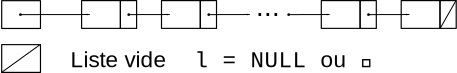
\includegraphics[scale=0.70]{../common-images/liste.pdf}}
	\end{block}
	\begin{block}{Déclarations}
		\begin{minted}[mathescape=true,escapeinside=||]{text}
|\underline{type}| Ptcellulle = |\underline{Pointeur de}| Cellule

|\underline{type}| Cellule = |\underline{structure}|
	valeur : <T>
	suivant : Ptcellule
|\underline{fin}|

|\underline{type}| Liste_chaînée = Ptcellule

l : Liste_chaînée
		\end{minted}
	\end{block}
\end{frame}


\begin{frame}[fragile=singleslide]
	\frametitle{Les listes chaînées :\\ Notation sur les pointeurs}
	\begin{block}{} %Notation algorithmique sur les pointeurs}
		\begin{itemize}
			\item \texttt{p$\uparrow$} : Cellule  $\Rightarrow$ Pointeur de Cellule
			\item \texttt{p$\uparrow$$\bullet$valeur}
			\item \texttt{p$\uparrow$$\bullet$suivant}
			\item \texttt{NULL} $\Rightarrow$ pointeur vide
		\end{itemize}
	\end{block}
	\vspace{1cm}
	\begin{block}{On trouve souvent la notation p->valeur à la place de p$\uparrow$$\bullet$valeur} %Notation algorithmique sur les pointeurs}
	\end{block}
\end{frame}

\begin{frame}[fragile=singleslide]
	\frametitle{Les listes chaînées :\\ Gestion dynamique des cellules}
	\begin{block}{} %Notation algorithmique sur les pointeurs}
		\begin{itemize}
			\item \texttt{\underline{Fonction} allouer() : Ptcellule}
			\begin{itemize}
				\item Fonction qui alloue dynamiquement une cellule 
				\item Résultat : pointeur sur la cellule allouée
			\end{itemize}
			\item \texttt{\underline{Action} libérer(p)}
			\begin{itemize}
				\item Récupère la cellule mémoire pointée par p
				\item Valeur de p ???
			\end{itemize}
		\end{itemize}
	\end{block}
\end{frame}


\begin{frame}[fragile=singleslide]
	\frametitle{Les listes chaînées --- Recherche}
	\begin{block}{SD essentiellement séquentielle $\Rightarrow$ parcours séquentiel} %Notation algorithmique sur les pointeurs}
		\begin{itemize}
			\item Par position
			\begin{itemize}
				\item Parcours du chaînage jusqu'au kième élément \\
                (coût = k)
			\end{itemize}
			\item Par valeur
			\begin{itemize}
				\item Séquentielle (coût min : 1, max : N)
				\item Séquentielle ordonnée (coût min : 1, max : N)
				\item Pas de dichotomie possible
			\end{itemize}
		\end{itemize}
	\end{block}
\end{frame}


\begin{frame}[fragile=singleslide]
	\frametitle{Les listes chaînées --- Parcours séquentiel}
	\vspace{-0.7cm}
	\begin{block}{} %{Exemple \small(moyennant les déclarations précédentes)}
		\begin{minted}[mathescape=true,escapeinside=||,fontsize=\footnotesize]{text}
|\underline{type}| Ptcellulle = |\underline{Pointeur de}| Cellule
|\underline{type}| Cellule = |\underline{structure}|
	valeur : <T>
	suivant : Ptcellule
|\underline{fin}|
|\underline{type}| Liste_chaînée = Ptcellule
		\end{minted}
		\begin{minted}[mathescape=true,escapeinside=||,linenos]{text}
|\underline{Action}| affich (l)
	|\underline{D}| : l : Liste_chaînée 
	|\underline{L}| : p : PtCellule
	p |$\leftarrow$| l
	|\underline{TQ}| p |$\ne$|  NULL |\underline{Faire}| 
		ecrire(p|$\uparrow$$\bullet$|valeur)
		p |$\leftarrow$| p|$\uparrow$$\bullet$|suivant
	|\underline{FTQ}|
|\underline{Faction}|
		\end{minted}
	\end{block}
\end{frame}


\begin{frame}[fragile=singleslide]
	\frametitle{Les listes chaînées --- Mises à jour}
	\vspace{-2cm}
	\begin{itemize}
		\item Ajout / Suppression de cellules
		\begin{itemize}
%			\item Ajout / Suppression de cellules
			\item Modification locale du chaînage
			\begin{itemize}
				\item Pas besoin de décalage de cellules
			\end{itemize}
		\end{itemize}
		\item Coût : constant \small(quelques affectations de pointeurs)
		\item Ajout dans une liste non ordonnée
		\begin{itemize}
			\item N'importe où, e.g en tête
		\end{itemize}
		\item Ajout dans une liste ordonnée
		\begin{itemize}
			\item Coût ???
		\end{itemize}
%		\item TODO: IMAGE
		
	\end{itemize}
\end{frame}

\begin{frame}[fragile=singleslide]
	\frametitle{Les listes chaînées --- Mise à jour \\\normalsize Ajout dans une liste non-ordonnée}
	\vspace{-0.7cm}
	\begin{block}{} %{Exemple \small(moyennant les déclarations précédentes)}
		\begin{minted}[mathescape=true,escapeinside=||,linenos,tabsize=4]{text}
|\underline{Action}| ajout_tête(l, val)
	|\underline{D}| : val : <T>
	|\underline{D/R}| : l : Liste_chaînée
	|\underline{L}| : p : Ptcellule
	
	p |$\leftarrow$| allouer()
	p|$\uparrow$$\bullet$|valeur |$\leftarrow$| val
	p|$\uparrow$$\bullet$|suivant |$\leftarrow$| L
	l |$\leftarrow$| p
|\underline{Faction}|
		\end{minted}
	\end{block}
	\begin{block}{Cas limite : liste vide}\end{block}	
\end{frame}

\begin{frame}[fragile=singleslide]
	\frametitle{Les listes chaînées --- Mises à jour \\\normalsize Ajout dans une liste ordonnée}
	\vspace{5cm}
%	\begin{block}{TODO: IMAGE} %Notation algorithmique sur les pointeurs}
%	\end{block}
	\begin{block}{Rechercher \texttt{prec}, pointeur précédent tel que}
		\begin{itemize}
				\item \texttt{prec$\uparrow$$\bullet$valeur $<$ val $\leq$ prec$\uparrow$$\bullet$suivant$\uparrow$$\bullet$valeur}
		\end{itemize}
	\end{block}
\end{frame}

\begin{frame}[fragile=singleslide]
	\frametitle{Les listes chaînées --- Mise à jour \\\normalsize Ajout dans une liste ordonnée}
	\vspace{-0.7cm}
	\begin{block}{} %{Exemple \small(moyennant les déclarations précédentes)}
		\begin{minted}[mathescape=true,escapeinside=||,linenos,tabsize=4]{text}
|\underline{Action}|  ajout_après ( prec, val)
	|\underline{D}| : prec : Ptcellule, val : <T>
	|\underline{L}| : p : Ptcellule

	p |$\leftarrow$| allouer()
	p|$\uparrow$$\bullet$|valeur |$\leftarrow$| val
	p|$\uparrow$$\bullet$|suivant |$\leftarrow$| prec|$\uparrow$$\bullet$|suivant
	prec|$\uparrow$$\bullet$|suivant |$\leftarrow$| p
|\underline{Faction}|
		\end{minted}
	\end{block}
	\begin{block}{Cas limites}\end{block}
		\vspace{-0.6cm}
		\begin{itemize}
			\item ajout en queue : OK
			\item ajout en tête : pas de \texttt{prec} $\Rightarrow$ algo \texttt{ajout\_tête}
			\item liste vide : idem
		\end{itemize}
\end{frame}

\begin{frame}[fragile=singleslide]
	\frametitle{Les listes chaînées --- Mises à jour \\\normalsize Suppression}
		\vspace{6cm}
%	\begin{block}{TODO: IMAGE} %Notation algorithmique sur les pointeurs}
%	\end{block}
	\begin{block}{Rechercher la cellule précédant celle à supprimer, soit \texttt{prec}}
	\end{block}
\end{frame}

\begin{frame}[fragile=singleslide]
	\frametitle{Les listes chaînées --- Mise à jour \\\normalsize Suppression}
	\vspace{-0.7cm}
	\begin{block}{} %{Exemple \small(moyennant les déclarations précédentes)}
		\begin{minted}[mathescape=true,escapeinside=||,linenos,tabsize=4]{text}
|\underline{Action}|  sup_après ( prec )
	|\underline{D}| : prec : Ptcellule
	|\underline{L}| : p : Ptcellule

	p |$\leftarrow$| prec|$\uparrow$$\bullet$|suivant
	prec|$\uparrow$$\bullet$|suivant |$\leftarrow$| p|$\uparrow$$\bullet$|suivant
	libérer (p)
|\underline{Faction}|
		\end{minted}
	\end{block}
	\begin{block}{Cas limites}\end{block}
		\vspace{-0.6cm}
		\begin{itemize}
			\item en queue : ok
			\item en tête : pas de prec $\Rightarrow$ \texttt{action sup\_tête}
		\end{itemize}
\end{frame}


\begin{frame}[fragile=singleslide]
	\frametitle{Les listes chaînées --- Mise à jour \\\normalsize Suppression}
	\vspace{-0.7cm}
	\begin{block}{} %{Exemple \small(moyennant les déclarations précédentes)}
		\begin{minted}[mathescape=true,escapeinside=||,linenos,tabsize=4]{text}
|\underline{Action}|  sup_tête ( l )
	|\underline{D/R}| : l : Liste_chaînée
	|\underline{L}| : p : Ptcellule

	p |$\leftarrow$| l
	l |$\leftarrow$| l|$\uparrow$$\bullet$|suivant
	libérer (p)
|\underline{Faction}|
		\end{minted}
	\end{block}
%	\begin{block}{Cas limites}\end{block}
%		\vspace{-0.6cm}
%		\begin{itemize}
%			\item en queue : ok
%			\item en tête : pas de prec $\Rightarrow$ \texttt{action sup\_tête}
%		\end{itemize}
\end{frame}


% % % % % % % % % % % % % % % % % % % % % % % % % % %
% END
% % % % % % % % % % % % % % % % % % % % % % % % % % %
\end{document}


% % % % % % % % % % % % % % % % % % % % % % % % % % %
% END
% % % % % % % % % % % % % % % % % % % % % % % % % % %

	\vspace{-0.9cm} \begin{center} \noindent\makebox[\linewidth]{\line(2,0){500}} \end{center}  \vspace{-0.7cm}
	\vspace{-0.9cm} \begin{center} \noindent\makebox[\linewidth]{\rule{\paperwidth}{1.5pt}}  \end{center}  \vspace{-0.7cm}	
